\usetikzlibrary{calc}
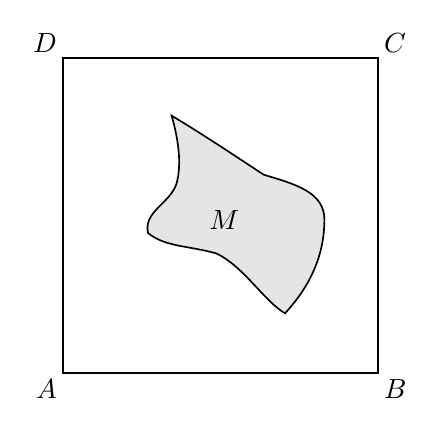
\begin{tikzpicture}[x=1cm,y=1cm,font=\normalsize,
  geometry edge/.style={solid,line width=.6pt},
  geometry label/.style={font=\normalsize,inner sep=2pt}]
  \coordinate (A) at (0,0);
  \coordinate (B) at (4,0);
  \coordinate (C) at (4,4);
  \coordinate (D) at (0,4);
  \draw[geometry edge] (A)--(B)--(C)--(D)--cycle;
  \draw[geometry edge,fill=gray!20] (1.38,3.27)
    .. controls (1.75,3.05) and (2.20,2.75) .. (2.55,2.52)
    .. controls (2.95,2.40) and (3.32,2.30) .. (3.32,1.95)
    .. controls (3.32,1.55) and (3.18,1.15) .. (2.82,0.76)
    .. controls (2.55,0.92) and (2.30,1.35) .. (1.95,1.52)
    .. controls (1.60,1.62) and (1.30,1.60) .. (1.08,1.78)
    .. controls (1.02,2.05) and (1.35,2.15) .. (1.44,2.40)
    .. controls (1.52,2.68) and (1.45,3.02) .. (1.38,3.27)
    -- cycle;
  \node[geometry label,below left] at (A) {$A$};
  \node[geometry label,below right] at (B) {$B$};
  \node[geometry label,above right] at (C) {$C$};
  \node[geometry label,above left] at (D) {$D$};
  \node[geometry label] at (2.05,1.95) {$M$};
\end{tikzpicture}
